\documentclass[a4paper,12pt]{article} 
\usepackage{geometry}
\usepackage{wrapfig}
\geometry{
	a4paper,
	total={170mm,257mm},
	left=10mm,
	right=10mm,
	top=20mm,
}
\usepackage{titlesec}
\titlelabel{\thetitle.\quad} %точка в section

%%% Работа с русским языком
\usepackage{cmap}                           % поиск в PDF
\usepackage{mathtext} 			 	       % русские буквы в формулах
\usepackage[T2A]{fontenc}               % кодировка
\usepackage[utf8]{inputenc}              % кодировка исходного текста
\usepackage[english,russian]{babel}  % локализация и переносы

%Математика
\usepackage{amsmath,amsfonts,amssymb,amsthm,mathtools} % AMS
\usepackage{icomma} % "Умная" запятая

%% Шрифты
\usepackage{euscript}	 % Шрифт Евклид
\usepackage{mathrsfs} % Красивый матшрифт

\usepackage{mathtext} 
\usepackage{setspace}
\usepackage{tabularx}
\usepackage{longtable}
\usepackage{icomma}
\usepackage{euscript}
\usepackage{float}
\usepackage{cutwin}
\usepackage{mathrsfs}
\usepackage{adjustbox}
\usepackage{dashbox}
\usepackage[normalem]{ulem}	
\usepackage[babel=true]{microtype}
\RequirePackage[T1]{fontenc}
\usepackage{amsmath,amsfonts,amssymb,amsthm,mathrsfs,mathtools} 
\usepackage{xcolor}         
\usepackage{enumitem}     
\usepackage{xpatch}       
\usepackage{cancel}                  
\usepackage{upgreek}                 
\usepackage{lipsum}                  
\usepackage[version=4]{mhchem}       
\usepackage{multirow}                
\usepackage{stackengine}             
\usepackage{tikz}         
\usepackage{hyperref}
\hypersetup{colorlinks=true,urlcolor=blue}       
\usetikzlibrary{positioning}         
\usepackage{titletoc}                 
\usepackage{chngcntr}              
\usepackage{fancyhdr}                
\usepackage{makecell}                
\usepackage{indentfirst}             
\usepackage{tocloft}                 
\usepackage{soul}                   
\usepackage[stable]{footmisc}       
\usepackage{subfig}                  

\mathtoolsset{showonlyrefs=true}


\theoremstyle{definition}
\newtheorem*{definition}{Определение}
\newtheorem{statement}{Предложение}[section]
\newtheorem{lemma}{Лемма}[section]
\newtheorem{theorem}{Теорема}[section]
\newtheorem*{theoremn}{Теорема}
\newtheorem*{corollary}{Следствие}
\newtheorem*{example}{Пример}
\newtheorem*{note}{Замечание}
\newtheorem*{problem}{Задача}


\counterwithout{footnote}{section}\DeclareRobustCommand{\divby}{%
	\mathrel{\text{\vbox{\baselineskip.65ex\lineskiplimit0pt\hbox{.}\hbox{.}\hbox{.}}}}%
}

\newcommand{\dotpr}[2]{\bra{#1}\ket{#2}}
\let\AA\relax
\let\emptyset\varnothing
\DeclareMathOperator*{\esssup}{ess sup}
\DeclareMathOperator*{\ord}{ord}
\DeclareMathOperator*{\supp}{supp}
\DeclareMathOperator*{\pr}{pr}
\DeclareMathOperator*{\Ker}{Ker}
\DeclareMathOperator*{\Vol}{Vol}
\DeclareMathOperator*{\rg}{rk}
\DeclareMathOperator*{\Ima}{Im}
\DeclareMathOperator*{\Alt}{Alt}
\DeclareMathOperator*{\Sym}{Sym}
\newcommand{\eqdef}{\stackrel{\text{\tiny{def}}}{=}}
\newcommand{\pp}{\partial}
\newcommand{\AA}{\mathcal{A}}
\newcommand{\BB}{\mathcal{B}}
\newcommand{\MM}{\mathbb{M}}
\newcommand{\NN}{\mathbb{N}}
\newcommand{\ZZ}{\mathbb{Z}}
\newcommand{\QQ}{\mathbb{Q}}
\newcommand{\RR}{\mathbb{R}}
\newcommand{\CC}{\mathbb{C}}
\newcommand{\FFF}{\mathbb{F}}
\newcommand{\DD}{\mathcal{D}}
\newcommand{\FF}{\mathcal{F}}
\newcommand{\sS}{\mathcal{S}}
\newcommand*\circled[1]{\tikz[baseline=(char.base)]{
		\node[shape=circle,draw,inner sep=2pt] (char) {#1};}}

%%% Заголовок
\author{Шилов Артем Б01-306}
\title{Лабораторная работа 3.2.5 \\
	\textbf{Свободные и вынужденные колебания в электрическом контуре}}
\date{\today}

\begin{document}
	
{\Large \maketitle}


\section{Ход работы}
\subsection{Измерение периодов свободных колебаний}
Соберем установку с рисунка 1, выставим $R=0$ Ом, $L=100$ мГн, $C=0$ нФ,  однако контур сам по себе обладает некоторым $C_0$, благодаря которому в контуре реализуются свободные колебания \par
Измерим с помощью осцилографа период затухающих колебаний 10T = 656 мкс, по периоду колебаний вычисляем значение емкости $C_0$, по формуле
$$C_0=\frac{T^2}{4\pi^2L}=1,09\,\text{нф}$$
Изменяя емкость C проведем измерения 10 периодов \\
\begin{center}
\begin{tabular}{|c|c|c|c|c|c|c|} \hline
    $C$, нф & 1.09& 2.09 & 4.09 & 6.09& 8.09&  10.09 \\ \hline
    $T$, мкс & 65.6& 90.8&127.0 &155.1 &178.8 &199.7   \\ \hline
    $T_{theor}$, мкс & 65.6 & 90.8 & 127.1 & 155.1& 178.7 & 199.6  \\ \hline
\end{tabular}
\end{center}
\subsection{Критическое сопротивление и декремент затухания}
Рассчитаем C, при котором собственная частота колебаний $\nu=1/(2\pi \sqrt{LC})=6500$\,Гц, $C=6$\,нф. Для выбранных L и С расчитаем критическое сопротивление контура $R_{cr}=8168$\,Ом по формуле $R_{cr}=2\sqrt{L/C}$  \par
Установим на магазине емкость, близкую к расчитанной увеличивая сопротивление до критической, пронаблюдаем картину затухающих колебаний. При сопротивлении $R=6$\,кОм колебательный режим переходит в апериодический. \par
Измения сопротивление запишем зависимость логарифмического декремента от сопротивления \par
\begin{center}
    \begin{tabular}{|c|c|c|c|c|c|c|} \hline
       R,\text{Ом}  & 410& 600& 800 &1000 &1200 & 1600\\ \hline
       $U_1$ & 588 & 660 & 470 & 610 & 360 & 550  \\
       $U_2$ & 400 & 370 & 250 & 250 & 150 & 140 \\
       $U_3$ & 284 & 220 & 140 & 100 & 70 & 40  \\
       $U_4$ & 192 & 130 & --- & 40 & ---& --- \\ \hline
       $\theta$  & 0.35 & 0.54 & 0.61 & 0.91 & 0.82 & 1.31  \\ \hline
    \end{tabular}
\end{center}
\subsection{Свободное колебание на фазовой плоскости}
Проведем аналогичные измерение, но уже на фазовой плоскости и запишем результату в таблицу. \par
\begin{center}
    \begin{tabular}{|c|c|c|c|c|c|c|} \hline
       R,\text{Ом}  & 410& 600& 800 &1000 &1200 & 1600\\ \hline
       $U_1$ & 21 & 20 & 20 & 19 & 18 & 17  \\
       $U_2$ & 14 & 12 & 10 & 8 & 6 & 4 \\
       $U_3$ & 10 & 7 & 5 & 3 & 2 & 1 \\ \hline
       $\theta$  & 0.37 & 0.52 & 0.69 & 0.92 & 1.10 & 1.42  \\ \hline
    \end{tabular}
\end{center}
\subsection{Исследование резонансных кривых}
Выставим значение емкости $C = 6$ нф и сопротивление $R = 410$ Ом (на этом моменте мы вспомнили,что забыли про $C_0$ и не учитывали его в течение всей лабораторной работы, поэтому нужно пересчитать частоту, $\nu_{res}=6015$\,Гц, критическое сопротивление $R_{cr}=7511$\,Ом)\par
Изменяя частоту генератора вблизи резонансной частоты, находим резонансную частоту $\nu = 6010$ Гц и ее амплитуду $2U_{res} = 16.7$\,B. \par
Снимем АЧХ вблизи резонанса \par
\begin{center}
    \begin{tabular}{|c||c|c|c|c|c|c|c|} \hline
        $\nu$,\,Гц & 5300 & 5390& 5480 & 5570 & 5660 & 5750 & 5840\\ \hline
        $2U$,\,B & 7 & 7.8 & 8.9 & 10.2 & 11.7 & 13.7 & 15.2 \\ \hline \hline
        $\nu$,\,Гц & 5930 & 6020& 6110 & 6200 & 6290 & 6380 & 6470 \\ \hline
        $2U$,\,B & 16.4 & 16.6 & 16.2 & 15 & 13.8 & 12.6 & 11\\ \hline \hline
        $\nu$,\,Гц & 6560 & 6650 & 6740 & 6830 & 6920 & 7010 & 7100 \\ \hline
        $2U$,\,B & 10.2 & 9.4 & 8.5 & 8.1 & 7.7 & 7.1 & 6.7 \\ \hline
    \end{tabular}
\end{center}

\subsection{Обработка результатов}
\textbf{1}. Из секции 3.1 построим график $T_{exp}=f(T_{theor})$
\begin{figure}[H]
    \centering
    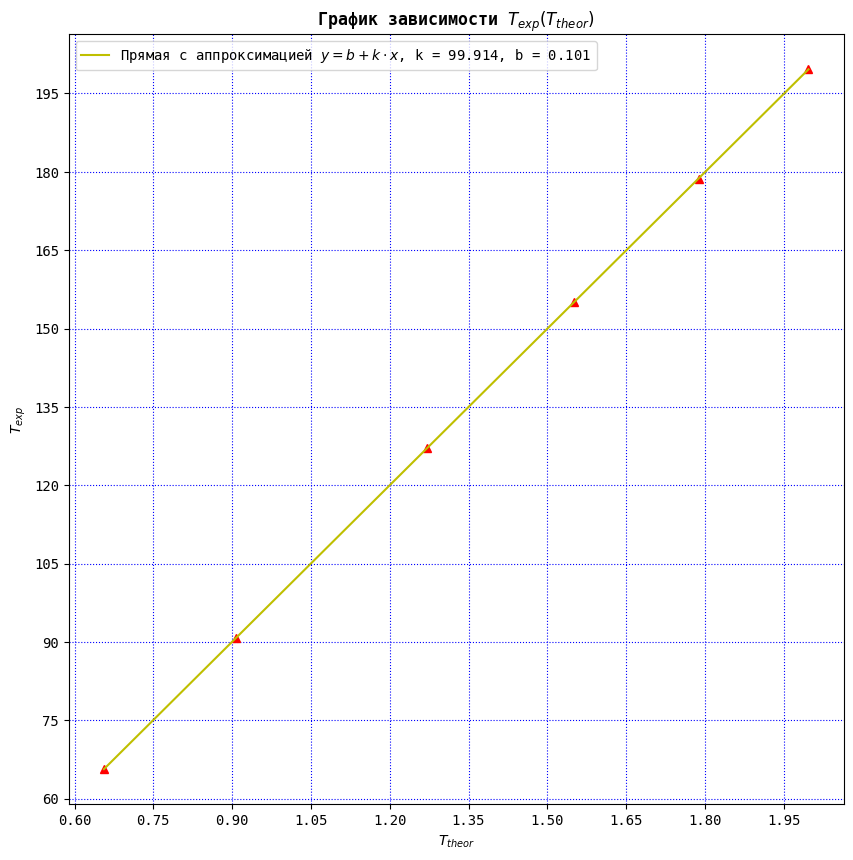
\includegraphics{324_1.png}    
\end{figure}
Из графика видно, что результаты совпали, погрешность $
<1\%$ \par
\textbf{2}.
Построим график $1/\theta^2=f[1/R^2]$
\begin{figure}[H]
    \centering
    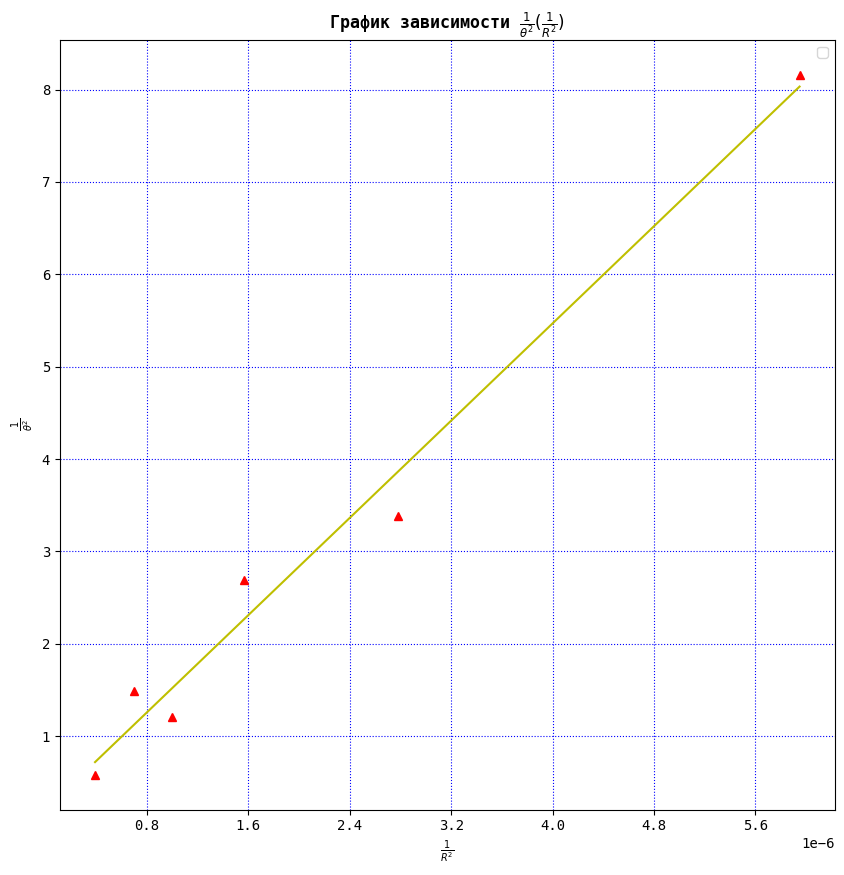
\includegraphics{324_2.png}    
\end{figure} \par
Коэффициент наклона $K=1320000 \pm 70000$\, Ом$^2$ \par
Зная коэффициент наклона, найдем $R_{cr}$, по формуле $R_{cr}=2\pi \sqrt{K}=7200 \pm 200$\,Ом, что близко с теоретическим значением $R_{cr}=7511$\,Ом \par
\textbf{3}. Расчитаем добротность для максимального и минимального значения $\theta$ и теоретическое с теми же параметрами.
\begin{itemize}
    \item Вычисление добротности контура по секции 3.2:\\
$$Q(\theta_{min})= 8.97 \qquad \qquad  Q(\theta_{max})= 2.40  $$
\item Вычисление добротности контура по секции 3.3:\\
$$Q(\theta_{min})= 8.49 \qquad \qquad  Q(\theta_{max})= 2.21  $$
    \item Вычисление добротности контура теоретически:\\   
$$Q(\theta_{min})= 9.16 \qquad \qquad  Q(\theta_{max})= 2.34  $$
\end{itemize}
\textbf{4}. По секции 3.4 построим АЧХ в масштабе $U/U_{res}=f(\nu /\nu_{res})$
\begin{figure}[H]
    \centering
    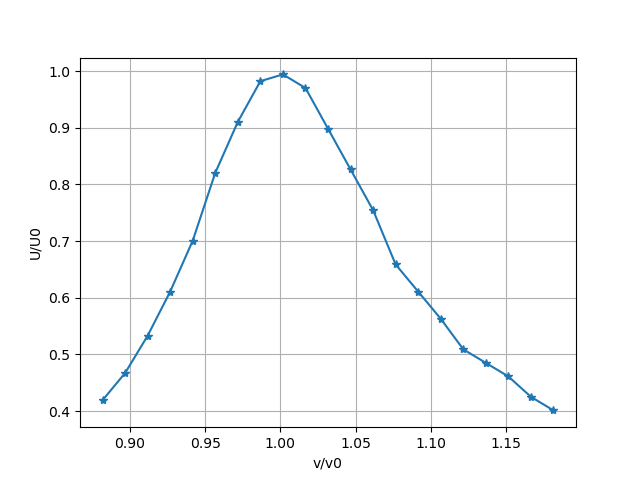
\includegraphics{324 3.png}    
\end{figure} \par
\textbf{5}. Рассчитаем добротность по формуле $Q=\nu_{res}/2\Delta \Omega$, Q=7.91
\section{Вывод}
В ходе эксперимента было установлено, что с учетом емкости системы экспериментальные значения периодов идеально совпадают с теоретически рассчитанными. Кроме того, удалось зафиксировать зависимость логарифмического декремента затухания от активного сопротивления цепи, при этом погрешность измерений составила около $5\%$. Критическое сопротивление, при котором колебания переходят в апериодический режим, было определено тремя методами: теоретически $R_{\text{кр}} = 7{,}5 \, \text{к}\Omega$, по наклону графика зависимости логарифмического декремента от сопротивления $R_{\text{кр}} = 7{,}2 \pm 0{,}2 \, \text{к}\Omega$, а также наблюдением за изменением характера колебаний $R_{\text{кр}} = 6 \, \text{к}\Omega$.
Результаты расчетов добротности сведены в таблицу: \\
    \begin{center}
        \begin{tabular}{|c|c|c|c|c|c|c|c|} \hline
             &\multicolumn{3}{c}{Свободные колебания} &\multicolumn{4}{|c|}{Вынужденные колебания} \\ \hline{}
           R, Ом & f(LCR) & f($\nu$) & Спираль& АЧХ & ФЧХ & Нарастание & Затухание\\ \hline
          410 &9.16 & 8.97& 8.49 & 7.91 & -& -&- \\ \hline
          1600 & 2.34 & 2.4& 2.21 & - & -& -&- \\ \hline
        \end{tabular}
            
    \end{center}

 Как видим, все добротности хорошо совпали.


\end{document}